\begin{figure}
    \caption{Evolución del recaudo del impuesto a la renta*}
    \label{fig:rentacree}
    \centering
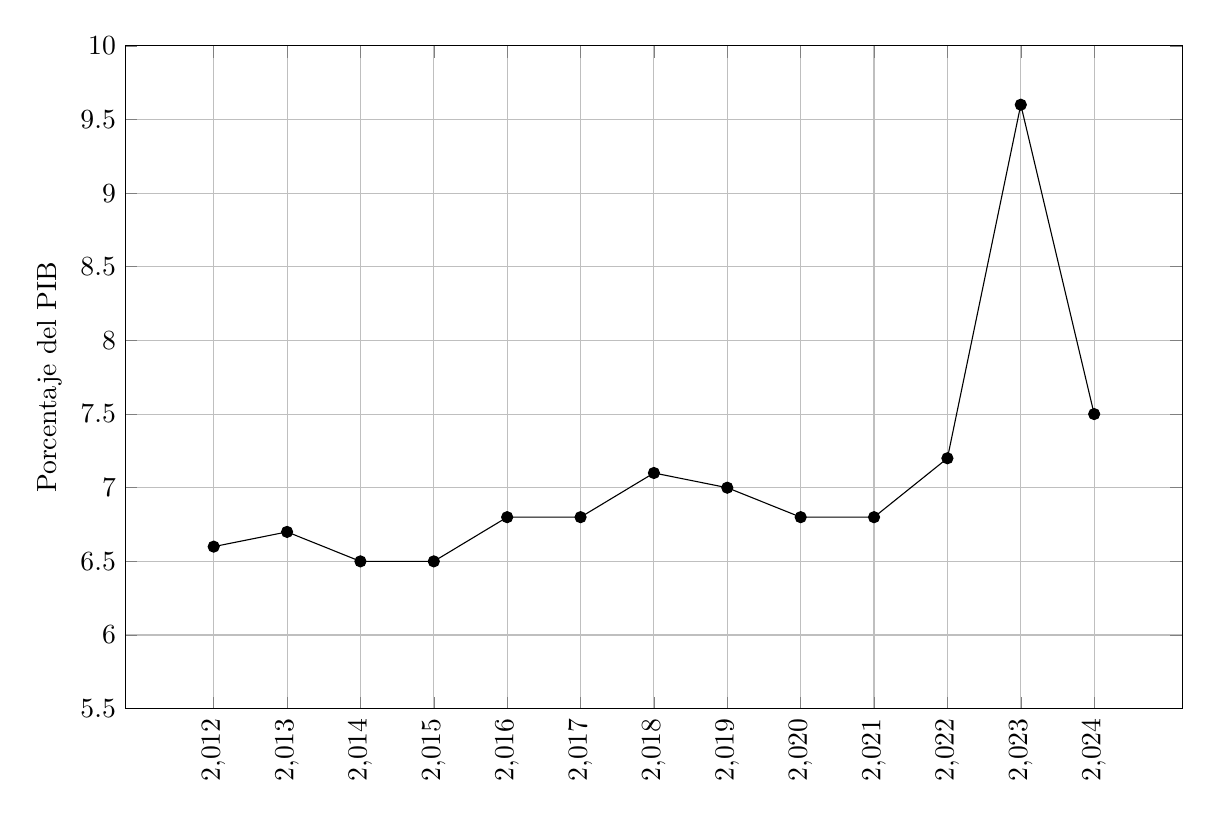
\begin{tikzpicture}
\begin{axis}[
    width=15cm,
    height=10cm,
%    xlabel={Año},
    ylabel={Porcentaje del PIB},
    grid=major,
    legend pos=north west,
    xtick=data,
    x tick label style={rotate=90, anchor=east},
    ymin=5.5,
    ymax=10,
    ytick={0, 0.5, 1, 1.5, 2, 2.5, 3, 3.5, 4, 4.5, 5, 5.5, 6, 6.5, 7, 7.5, 8, 8.5, 9, 9.5, 10}
]

\addplot[mark=*] coordinates {
%    (2011, 5.4)
    (2012, 6.6)
    (2013, 6.7)
    (2014, 6.5)
    (2015, 6.5)
    (2016, 6.8)
    (2017, 6.8)
    (2018, 7.1)
    (2019, 7.0)
    (2020, 6.8)
    (2021, 6.8)
    (2022, 7.2)
    (2023, 9.6)
    (2024, 7.5)    
};

%\legend{Renta + CREE}
\end{axis}
\end{tikzpicture}
\vspace{0.1cm}
\par \footnotesize{*Incluye recaudo del CREE entre 2013 y 2016.}
\vspace{0.1cm}
\par \footnotesize{\textit{Fuente: Balance General del GNC, Ministerio de Hacienda.}}
\end{figure}
